\chapter{Introduction}\label{chap:introduction}

\section{The Challenge of Environmental Pollution}

Over the past few decades, the upsurge in environmental pollution by chemical compounds has been driven by industrial processes, agricultural methods, our consumerism and various other contributing factors. Although these chemicals are integral for many products and have the potential to improve our comfort of modern society, they can also pose risks and adversely affect both our health and the environment, either acutely or chronically. Toxic substances threaten wildlife but also make our air, soil and finally our drinking water and food supply less safe. 

The EU maintains comprehensive chemical regulations, however, it is anticipated that global chemicals production will double by 2030~\cite{chemicaloutlook}. Moreover, the widespread utilization of chemicals, including their inclusion in consumer goods, is expected to expand further.
Even though there are over 275 million known chemical compounds registered by the \emph{Chemical Abstracts Service}~\cite{CAS}, merely a tiny fraction of them undergo close monitoring via target analytical approaches and even less is known about their toxicity profiles and negative health effects on our organsims. Table~\ref{tab:ubiquitous_water_pollutants} provides an overview of omnipresent water pollutants.

\begin{table}[h]
    \begin{tabularx}{\linewidth}{XXXX}
    \toprule
    Origin/Usage & Class & Examples & Related Issues \\
    \toprule
    Industrial\newline Chemicals & Solvents & Tetrachloro-methane & Drinking-water-quality \\
    & Intermediates & Methyl-t-butylether & Drinking-water-
    quality \\ 
    & Petrochemicals & BTEX (benzene, toluene, xylene) & Cancer \\ \midrule
    Industrial\newline Products & Additives & Phthalates & Endocrine disruptors \\
     & Lubricants & PCBs & Biomagnification \\
     & Flame Retardants & PBDEs & \\ \midrule
    Consumer\newline Products & Detergents & Nonylphenol ethoxylates & Endocrine effects \\
     & Pharmaceuticals & Antibiotics & Bacterial resistance \\
     & Hormones & Ethinyl estradiol & Feminization of fish \\ \midrule
     Biocides & Pesticides & DDT & Toxic effects and persistent metabolites \\
     & Nonagricultural biocides & Tributyltin & Endocrine effects \\ \midrule
    Geogenic \& \newline Natural\newline Chemicals & Heavy Metals & Lead, cadmium, mercury & Organ damage \\
     & Inorganics & Arsenic, selenium, fluoride & Drinking-water-quality\\
     & Taste and Odor & Geosmin & \\
     & Human Hormones & Estradiol & Feminization of fish \\ \midrule
    Disinfection \& \newline Oxidation & Disinfection by-products & Haloacetic acids, Bromate & Drinking-water-quality \\ \midrule
     Transformation Products & Metabolites from all above & Metabolites of perfluorinated compounds & Bioaccumulation\\
     & & Chloroacetanilide herbicide metabolites & Drinking-water-quality \\
    \bottomrule
    \end{tabularx}
    \caption{Table 2 adapted from~\cite{schwarzenbach2006}. Examples of ubiquitous water pollutants.}~\label{tab:ubiquitous_water_pollutants}
\end{table}

Building upon the \emph{European Green Deal}~\cite{greendeal} and the \emph{8th Environment Action Programme}, which guides European environmental policy until 2030, reinforces the EU's goal of sustainable living within planetary limits, with a vision extending to 2050. One of its key objectives is a zero-pollution commitment, covering air, water, and soil, prioritizing the well-being of EU citizens. In particular, the \emph{European Commission} published a sustainability-focused chemicals strategy, aligning with the EU's zero-pollution ambition with one of the objectives to minimize concerning substances by either substituting or phasing them out wherever feasible~\cite{EUChemicalsStrategy}. 
Consequently, the urgent need to monitor and effectively assess the hazards associated with the daily entering of thousands of poorly understood chemicals into our environment becomes increasingly evident.

\section{The Imperative for Prioritization and Toxicity Assessment}

Contemporary analytical techniques, particularly \emph{high-resolution mass spectrometry (HRMS/MS)}, are gaining significance across various domains such as metabolomics, drug discovery, forensics, environmental science, and toxicology.~\emph{Nontarget HRMS/MS} has improved the ability to detect emerging compounds in environmental samples, often with unknown toxicity profiles. These compounds are assessed based on factors such as abundance and fragmentation data. However, the task of identifying compounds and understanding their toxicity continues to be demanding in terms of resources and time. Additionally, the scarcity of thoroughly characterized reference substances for comparison when studying unknown compounds adds complexity, making it difficult to achieve comprehensive elucidation. Traditionally, the prioritization of unidentified compounds rely on signal intensity as a guiding metric. Unfortunately, this approach falls short in delivering an accurate assessment of environmental exposures, as it tends to overlook the crucial toxicological dimension. As a result, substances with the potential for severe ecological consequences, such as endocrine-disrupting compounds, often go undetected because of their low abundance, even though they exhibit high levels of toxicity. Hence, a pressing requirement exists for alternative approaches to prioritize unidentified \emph{NTS HRMS/MS} signals based on their hazard potential, which can better incorporate considerations of toxicity and ecological consequences. Figure~\ref{fig:non_target_high_resolution_mass_spectrometry} illustrates the non-target screening with \emph{HRMS/MS} technique and the novel prioritization approach.

\begin{figure}[htbp]  % Placement options: h (here), t (top), b (bottom), p (page)
    \centering
    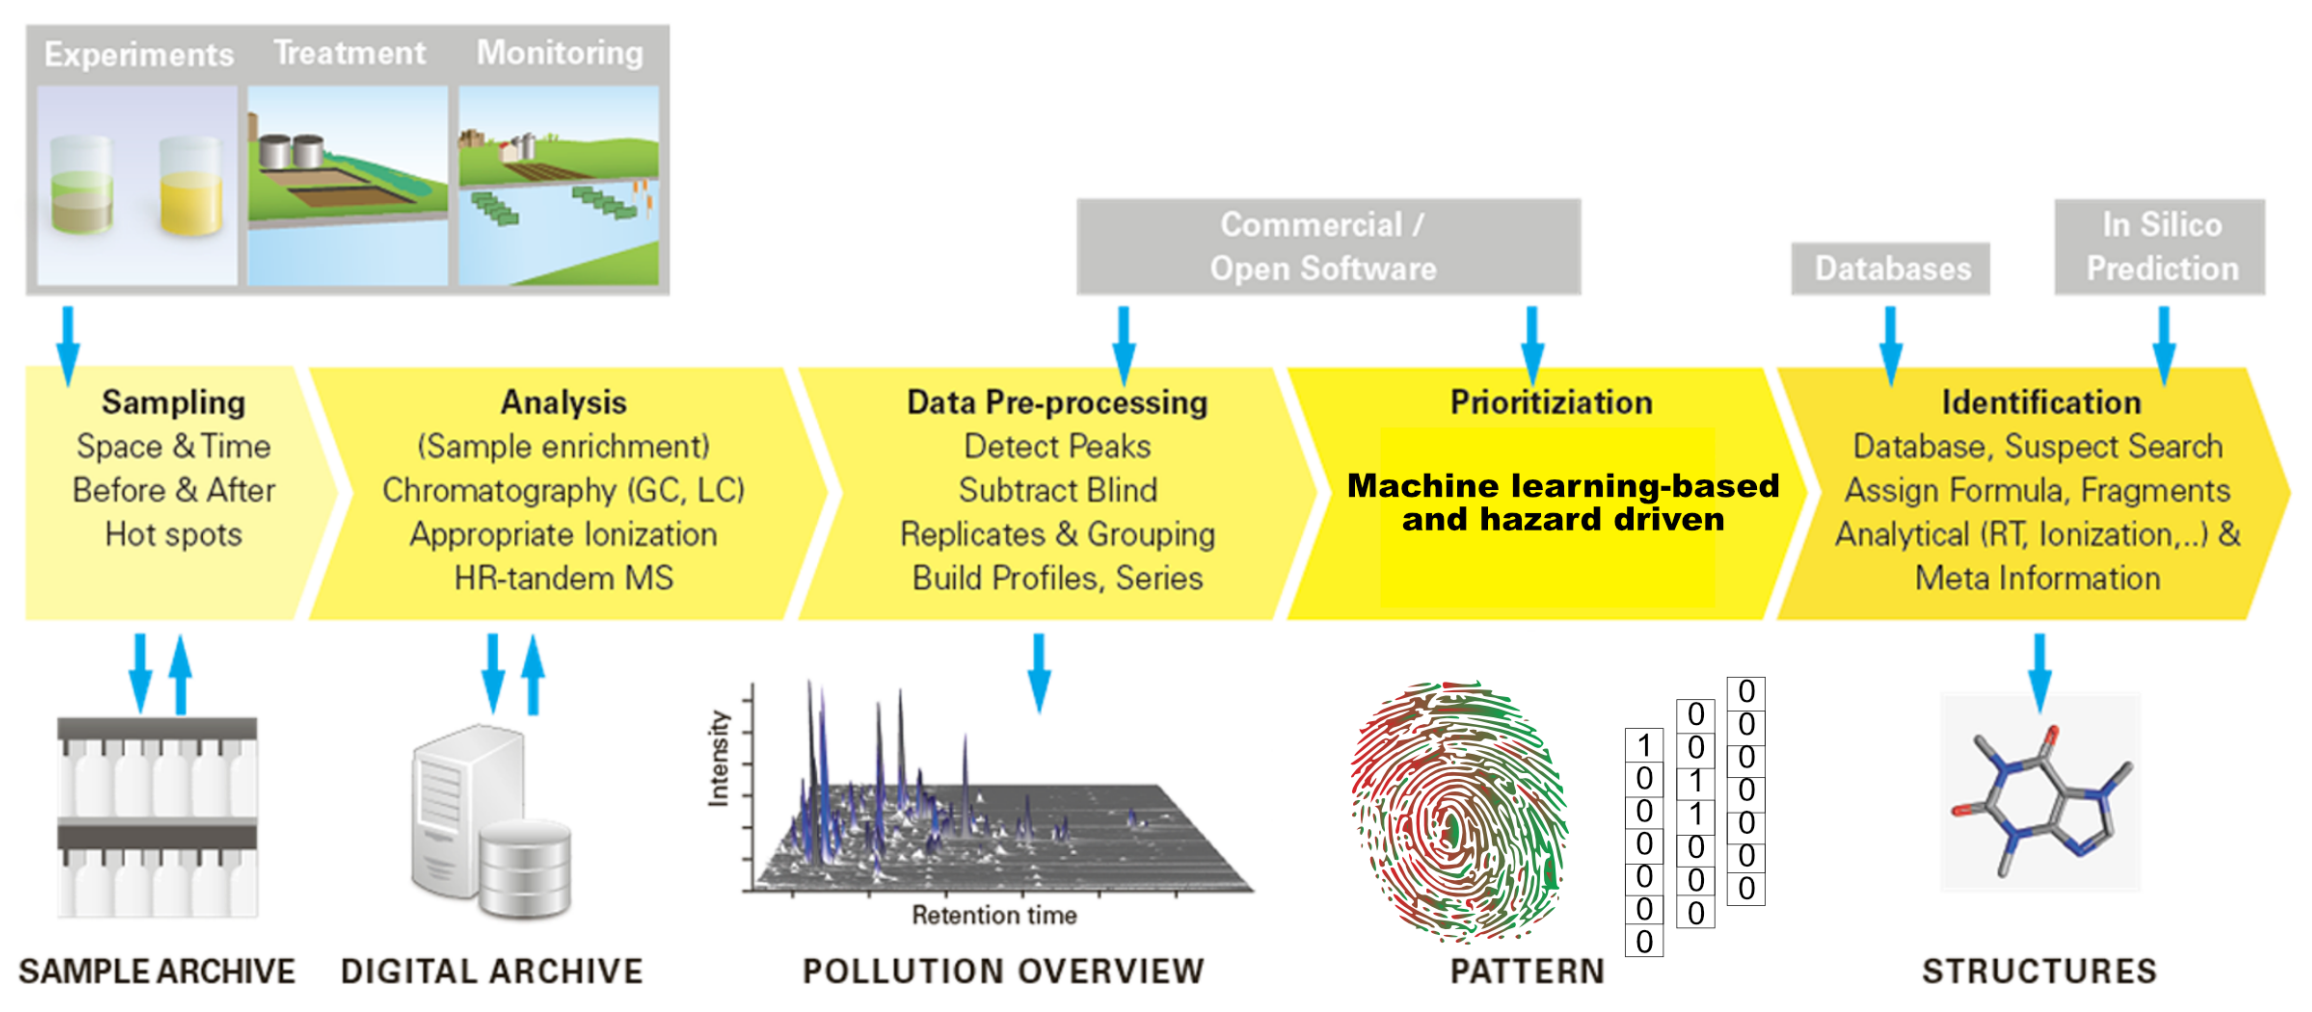
\includegraphics[width=1.0\textwidth]{figures/non_target_high_resolution_mass_spectrometry_1.png}  
    \caption{Figure 1 adapted (with modified Prioritization step) from Hollender et al.~\cite{hollender}: Nontarget screening with high resolution mass spectrometry in the environment: Ready to go? }
~\label{fig:non_target_high_resolution_mass_spectrometry} 
\end{figure}

\section{Unlocking the Potential of High-Throughput Screening and Machine Learning in Toxicity Prediction}

In the past few years, the use of machine learning methods has emerged as a transformative force in the field of \emph{in vitro} toxicology, particularly in the realm of high-throughput toxicity prediction. High-throughput screening (HTS) has revolutionized the way we assess toxicity by allowing thousands of \emph{in vitro} bioassays to be conducted efficiently. This high-throughput approach, coupled with advancements in robotics and automated analysis, has generated large volumes of toxicity data, paving the way for more comprehensive assessments of chemical compounds.
Alongside the rise of machine learning, this advancement has facilitated the creation of predictive models capable of forecasting compound toxicity based on their chemical structure~\cite{banerjee2018}. These models can be trained on extensive datasets containing well-documented toxicity information, allowing them to learn the underlying patterns and relationships between chemical structures and target toxicity. Once trained, these models can predict the toxicity of new compounds, even if they have not undergone laboratory testing. This approach holds the potential to significantly reduce the time and cost associated with early-stage toxicity pre-assessment and plays a crucial role in prioritizing compounds for further in-depth testing.

\begin{figure}[htbp]
    \centering
    \begin{subfigure}[b]{0.48\textwidth}
        \centering
        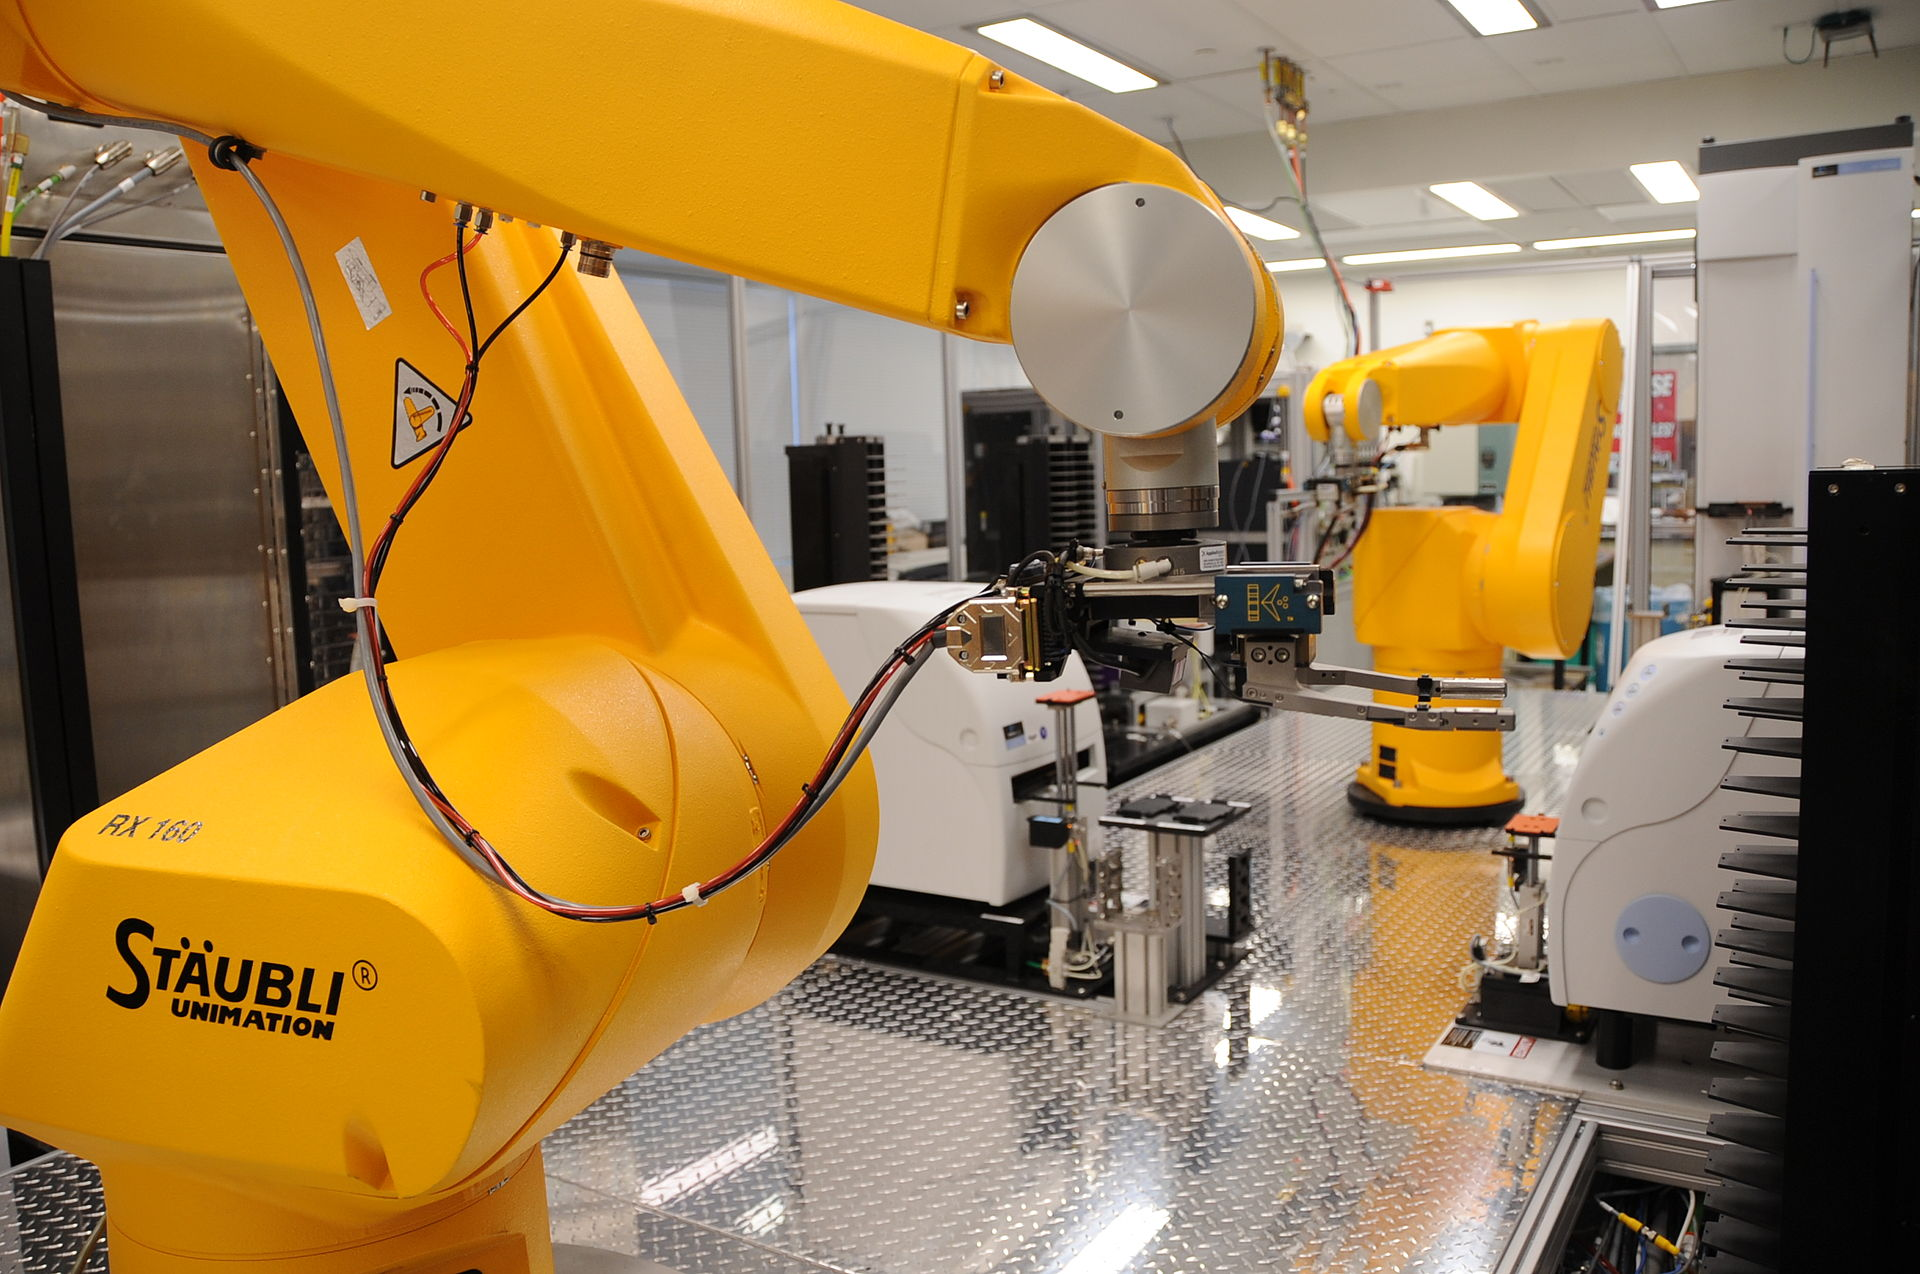
\includegraphics[width=\textwidth]{figures/hts_robot.png}
        \caption{A robot arm retrieves assay plates from incubators and places them at compound transfer stations or hands them off to another arm that services liquid dispensers or plate readers. Efforts in the automation, miniaturization and the readout technologies have enabled the growth of HTS. Image obtained from~\cite{hts_robot}}
        \label{fig:hts_robot}
    \end{subfigure}
    \hfill
    \begin{subfigure}[b]{0.48\textwidth}
        \centering
        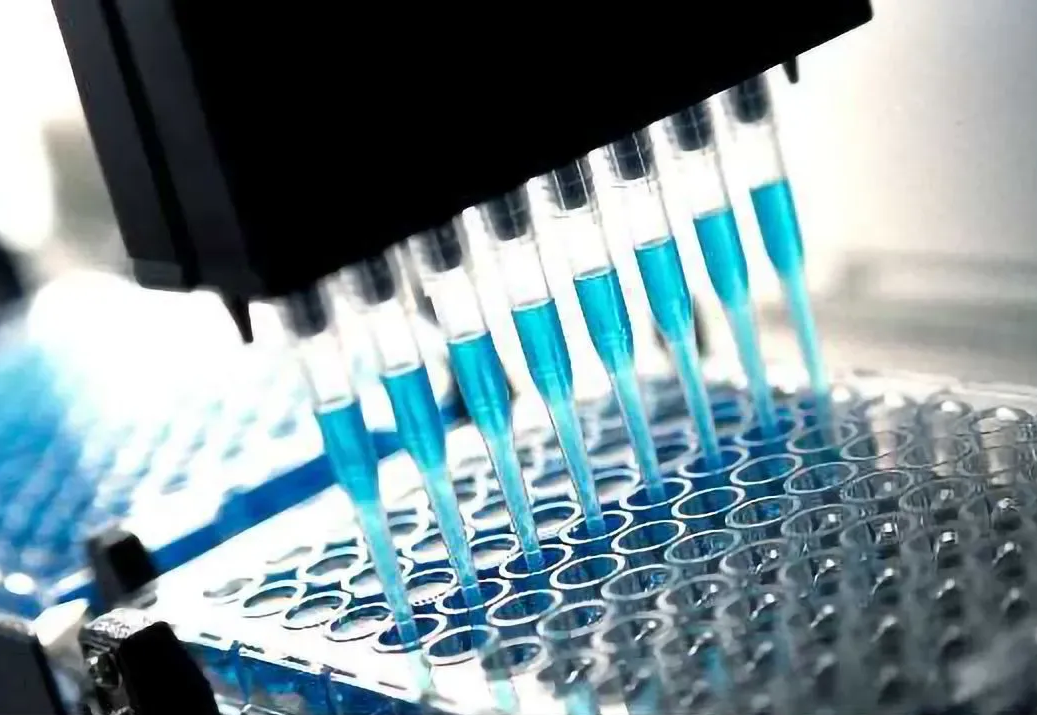
\includegraphics[width=\textwidth]{figures/hts.png}
        \caption{Modern microtitre assay plates consist of multiples of 96 wells, which are either prepared in the laboratory or acquired commercially from stock plates. These wells are filled with a dilution solvent, such as DMSO, along with any other chemical compounds intended for analysis. Image obtained from~\cite{hts_plates}}
        \label{fig:hts_plates}
    \end{subfigure}
    \caption{High-Throughput Screening (HTS)}
    \label{fig:hts}
\end{figure}


\section{MLinvitroTox: A Novel Approach}

In response to the pressing need for a more hazard-driven and comprehensive assessment of environmental contaminants, \emph{Arturi et al.} introduced \emph{MLinvitroTox}~\cite{arturi}, an innovative machine learning framework.
 The primary objective of this thesis is to collaborate with the authors to further enhance and advance this framework.~\emph{MLinvitroTox} leverages molecular fingerprints extracted from fragmentation spectra\footnote{also termed as \emph{Tandem mass spectrometry} or \emph{MS/MS} or \emph{MS2}}, marking a fundamental shift in how we forecast the toxicity of the myriad unidentified \emph{HRMS/MS} features. While traditional \emph{QSAR} models predict bioactivities based on molecular fingerprints derived from chemical structures, \emph{MLinvitroTox} was trained with supervised classification models on molcular fingerprints from chemical structures but is applied to molecular fingerprints generated from experimentally measured \emph{MS2} spectra using \emph{SIRIUS} and \emph{CSI:FingerID}~\cite{sirius2019}.~\emph{SIRIUS} is a software package for annotating small molecules from nontarget HRMS/MS data, while \emph{CSI:FingerID} is a machine-learning tool employed by \emph{SIRIUS} to predict molecular fingerprints from fragmentation spectra.~\emph{MLinvitroTox} leverages streamlined machine learning techniques to predict the compounds bioactivity, respectively toxicity, ensuring a broad toxicological coverage encompassing over 400 target-specific and 70 cytotoxic endpoints, sourced from \emph{ToxCast}/\emph{Tox21} data. Subsequently, the toxicity predictions generated by the framework are employed to prioritize compounds, with the flexibility to emphasize specific aspects of toxicity profiles tailored to individual preferences. This prioritization strategy facilitates more streamlined and thorough evaluations of environmental contaminants, enhancing a more hazard-driven risk assessment.


\section{Objectives and Significance}

The primary goal of this thesis is to contribute to the development of an efficient framework for predicting compound toxicity across multiple endpoints. The ultimate output of the pipeline are the toxicity fingerprints that encode the predicted toxcity from \emph{HRMS} environmental samples for the relevant endpoints of interest. The generated toxicity fingerprints will provide valuable insights for the prioritization process in identifying most hazardous compounds found in environmental samples, ultimately contributing to the preservation of ecosystems and our health. The framework aims to develop a custom processesing and curation of structural and toxicological data to address challenges from modeling heterogenuous and imbalanced data sets.

\section{Thesis Structure}

The initial chapters lay the groundwork by providing essential background information and summarizing related work. As we progress through the subsequent chapters, we will explore the materials and methods employed, providing insights into the technical intricacies of preparing ToxCast/Tox21 toxicity data and transforming them into appropriate inputs for our machine learning pipeline. This foundational work will serve as the cornerstone for the forthcoming chapters, where we will showcase the potential of \emph{MLinvitroTox}. Additionally, will also demonstrate the framework's effectiveness through validation using real-world mass spectral data from \emph{MassBank}~\cite{massbank} and discuss about the implications of our research.
